\documentclass[main.tex]{subfiles}

\begin{document}
	\chapter{Compléments de théorie des groupes}
	\section{Rappel sur les groupes libres}

	Dans ce chapitre, $G$ est un groupe et $I$ un ensemble, fini ou non. $F(I)$ dénote le groupe libre sur $I$. 
	\begin{example}
		Pour $I = \{\star\}$, $F(I) \cong \mathbf{Z}$, en effet si $x$ est le générateur, $$F(I) = \{x^{n} \;|\; n \in \mathbf{Z}\}.$$
		Pour $I = \{1,2\}$, $F(x,y)$ est le groupe formé de tous mes mots qu'on peut écrire avec $x$ et $y$ et leurs inverses $x^{-1}$, $y^{-1}$. Typiquement tout élément de $F(x,y)$ s'écrit comme  \[
		x^{k_1}y^{l_1}x^{k_2}\ldots \quad l_i, k_j \in \mathbf{Z} 
		.\] 
		La seule relation imposée sur la multiplication, ou juxtaposition, est que \[
			xx^{-1} = 1 = x^{-1}x \qquad \text{et} \qquad yy^{-1} = 1 = y^{-1}y
		.\] 
	\begin{remark}
		En général un groupe peut admettre \emph{plusieurs} présentations, par exemple le groupe trivial $\star$ admet une présentation `vide', mais aussi $\langle x \;|\; x^2,x^3 \rangle$.
	\end{remark}
	\end{example}
	\begin{prop}[Propriété universelle]
		Un homomorphisme $f : F(x,y) \longmapsto G$ correspond à la donnée de deux éléments dans $G$, les images de $x$ et $y$.
	\end{prop}
	\section{Présentation de groupes}
	Il est possible de définir un groupe par une \emph{présentation} qui lui est propre, c'est à dire la donnée d'un ensemble de générateurs et de relations que ceux-ci vérifient. Il s'agit d'un écriture compacte exprimant les propriétés fondamentales du groupe. \\
	Dans cette section $S \subset G$ dénote un sous ensemble qui engendre tout le groupe $G$. Ainsi si $S$ engendre $G$, il est possible d'écrire tout élément de $G$ comme un produit  \[
	x_1^{k_1}x_2^{k_2}\ldots x_n^{k_n}, \; x_i \in S, \; k_i \in \mathbf{Z} \; \; \forall i \in \{1,\ldots n\} 
	.\] 
	Si $G$ n'est pas libre, cette écriture n'est pas unique. Pour arriver à retrouver notre groupe $G$ il faut mettre en évidence certaines relations et montrer quels produits sont égaux. Il suffit pour cela de spécifier quels produits sont égaux à l'élément neutre de $G$. Il est bon de noter qu'il n'est en général pas nécessaire d'expliciter \emph{toutes} ces relations.

	\begin{definition}[Présentation de groupe]
		Pour un ensemble S, et $R \subset F(S)$	une partie du groupe libre, on appelle \emph{clôture normale} de $R$ le plus petit sous groupe distingué $N$ de $F(S)$ contenant $R$. On note le quotient $\quot{F(S)}{N} \eqdef \langle S \;|\; R \rangle$ et on dit que $G$ admet une représentation $\langle S \;|\; R \rangle$ s'il lui est isomorphe.
	\end{definition}

	Commençons par prendre un exemple simple pour illustrer cette notion, celui du groupe symétrique $S_{3} = \{1, (12), (13), (23), (123), (132)\}$. $S_{3}$ est engendré par les deux transpositions $(12), (23)$ ainsi nous avons un homomorphisme surjectif
	\begin{align*}
		\varphi : F(x,y) &\longmapsto S_3 \\
		x &\longmapsto (12) \\
		y &\longmapsto (23)
	.\end{align*}
	Le noyau est un sous groupe normal de $F(x,y)$ dont les générateurs sont donnés par les relations dans $S_{3}$ $(12)^2 = 1, \; (23)^2 = 1, \; ((12)(23))^3 = 1$. \\
	Soit maintenant $N \triangleleft F(x,y)$ engendré par $x^2,y^2,(xy)^3$
	\begin{prop}
		$\quot{F(x,y)}{N} \cong S_3$.
	\end{prop}
	\begin{proof}
		On a l'homomorphisme
		\begin{align*}
			\varphi : F(x,y) &\longmapsto S_{3} \\
			x &\longmapsto (12) \\
			y &\longmapsto (23)
		.\end{align*}
		On constate que $\varphi(N) = 1$ donc $\varphi$ passe au quotient et induit un homomorphisme surjectif  $\overline{\varphi} : \quot{F(x,y)}{N} \longmapsto S_{3}$. Pour voir que $\overline{\varphi}$ est injectif on compte les éléments. Les éléments du quotient $\quot{F(x,y)}{N}$ sont des classes de mots en $x$ et $y$. Or $x^2,y^2 \in N$, on peut choisir comme représentant de chaque élément du quotient ne faisant intervenir que $x$ et $y$ à la puissance 1. Ces mots sont de la forme $xyx\ldots xy$ ou $xyx\ldots yx$ ou $yxy\ldots yx$ ou $yxy\ldots xy$. Le dernier relateur est $(xy)^3 = xyxyxy \in N$, de fait dans le quotient $xyx = yxy$. Finalement on a $\quot{F(x,y)}{N} = \{ \overline{1}, \overline{x}, \overline{y}, \overline{xy}, \overline{yx}, \overline{xyx}\}$. Cela montre que $\varphi$ est injectif, c'est donc un isomorphisme.
	\end{proof}
	Ainsi on a identifié $S_{3} \cong \langle x,y \;|\; x^{2},y^{2},(xy)^{3} \rangle$ qui se lit comme le groupe engendré par $x,y$ avec les relations $x^2 = 1, y^2 = 1, (xy)^3 = 1$.
	\section{Le graphe de Cayley}
	\begin{definition}[Graphe de Cayley]
		Soit $S$ un ensemble de générateurs d'un groupe $G$, le graphe de Cayley $\Gamma = \Gamma(G,S)$ est le graphe coloré et orienté dont les sommets sont les éléments de $G$ et une arrête de couleur $s \in S$ relie $g$ à $g\cdot s$. 
	\end{definition}
	\begin{example}
		Si $G = C_2$ et $S = \{x\} $ où $x$ est le générateur on a une seule couleur et le graphe est le suivant. 
		Par convention, si $x$ est d'ordre 2 on peut simplifier l'écriture de ce graphe en utilisant une arrête \emph{non orienté} entre $g$ et $g\cdot x$.
		\begin{figure}[ht]
			\centering
			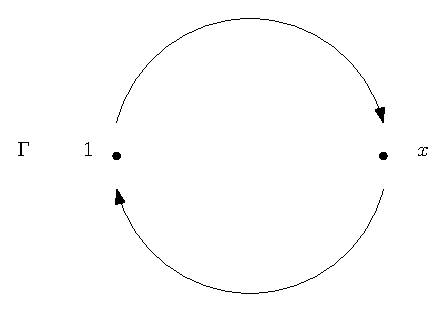
\includegraphics[width=0.5\textwidth]{cayley.eps}
			\caption{Illustration du graphe de Cayley pour $G = C_{2}$}
		\end{figure}
	\end{example}
	\begin{example}
		Cet exemple illustre la convention précédente, pour $G = \mathbf{Z}$ et $S = \{1\}, S' = \{1,-1\} $ alors les graphes $\Gamma(\mathbf{Z},S), \Gamma(\mathbf{Z},S')$ sont les suivants \\
		\bigskip

		\begin{minipage}{0.5\textwidth}
			\centering
			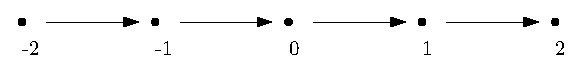
\includegraphics[width=0.8\textwidth]{cayleyZ.eps}
			\captionof{figure}{$\Gamma(\mathbf{Z},S)$}
		\end{minipage}
		\hfill
		\begin{minipage}{0.5\textwidth}
			\centering
			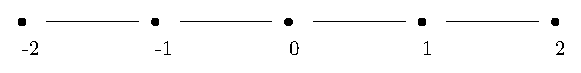
\includegraphics[width=0.8\textwidth]{cayleyZ2.eps}
			\captionof{figure}{$\Gamma(\mathbf{Z},S')$}
		\end{minipage}
		\bigskip

		Le fait que $-1$ soit dans $S'$ on peut lire chaque arrête dans les deux sens et donc le graphe n'est pas orienté. Lorsque les générateurs dans $S$ sont d'ordre infini il est préférable que $S$ contienne les inverses de ses générateurs.
	\end{example}
	\section{Produit libre}
	Dans cette section on considère deux groupes donnés par les présentations $G = \langle x_{\alpha} \;|\; r_{\beta} \rangle, \; \alpha \in I, \beta \in J$ et $H = \langle x_{\gamma} \;|\; r_{\delta} \rangle, \; \gamma \in K, \delta \in L$. \\
	$F(I)$ dénote le groupe libre dont les générateurs sont $x_{\alpha}$ et $F(K)$ le groupe libre dont les générateurs sont les $x_{\gamma}$.

	\begin{definition}[Produit libre]
		Le produit libre $G * H$ est le groupe donné par la présentation $\langle x_{\alpha}, x_{\gamma} \;|\; r_{\beta},r_{\delta} \rangle$.
	\end{definition}
	\begin{lemma}
		Il existe des morphismes injectifs
		\begin{align*}
			i : G &\longmapsto G*H \\
			j : H &\longmapsto G*H
		.\end{align*}
	\end{lemma}
	\begin{proof}
		Par symétrie de la construction du produit libre on ne s'occupe que de $i$. On considère la composition suivante
		\medskip

		\adjustbox{scale=0.8,center}{%
			\begin{tikzcd}
				F(I) \arrow[r] \arrow[dd]     & F(I\amalg K) \arrow[r] & G*H \arrow[r] & \quot{F(I\amalg K)}{r_{\beta} = 1 = r_{\gamma}} \\
							      &                        &               &   \\
				G = \quot{F(I)}{r_{\beta} = 1} \arrow[rrruu, "i"', dotted] &                        &               &  
			\end{tikzcd}
		}
		\medskip

		Cette composition passe au quotient puisque $r_{\beta}$ est envoyé sur 1 dans $G*H$. On appelle $i$ cet homomorphisme. Il reste alors à montrer l'injectivité.
		Il existe un autre homomorphisme surjectif 
		\begin{align*}
		\pi :	F(I\amalg K) &\longmapsto G \\
			x_{\alpha} &\longmapsto x_{\alpha} \\
			x_{\gamma} &\longmapsto 1
		.\end{align*}
		On observe que $\pi(r_{\beta}) = 1 = \pi(r_{\gamma})$ donc $\pi$ passe au quotient, donc 
		\begin{alignat*}{4}
			G &\xmapsto{i} G&&*H &&&\xmapsto{\overline{\pi}} G \\
			x_{\alpha} &\mapsto &&x_{\alpha} &&&\mapsto x_{\alpha}
		.\end{alignat*}
		Ainsi $\overline{\pi} \circ i = Id_G$ et en particulier $i$ est injectif.
	\end{proof}

	\begin{prop}[Propriété universelle]
		Nous énonçons la propriété universelle du produit libre \\

		\medskip
		\begin{minipage}{0.5\textwidth}
			Le diagramme suivant est un pushout, c'est à dire pour tous homomorphismes $\varphi : G \longmapsto M$ $\psi : H \longmapsto M$ il existe un unique morphisme $\omega : G*H \longmapsto M$ tel que $\omega \circ i = \varphi$ et $\omega \circ j = \psi$.
		\end{minipage}	
		\hfill
		\begin{minipage}{0.5\textwidth}
			\[
			\xymatrix@R=1.2cm@C=1.2cm{
			 1 \ar[r]      \ar[d]         & H \ar[d]_{j} \ar@/^1pc/[rdd]^{\psi}   \\
			 G \ar[r]^{i} \ar@/_1pc/[rrd]_{\varphi} & G*H \ar@{-->}[rd]_{\exists! \; \omega}             \\
							      &                                   & M 
			}
	\]
		\end{minipage}
	\end{prop}
	\medskip
	\begin{proof}
		On définit un homomorphisme $\Omega : F(I \amalg K) \longmapsto M$ par $\Omega(x_{\alpha}) = \varphi(x_{\alpha})$ et $\Omega(x_{\gamma}) = \psi(x_{\gamma})$. Cet homomorphisme passe au quotient. En effet $\Omega(r_{\beta}) = \varphi(r_{\beta}) = 1$ et $\Omega(r_{\gamma}) = \psi(r_{\gamma}) = 1$. On a bien $\omega \circ i = \varphi$ et $\omega \circ j = \psi$ puisque les $x_{\alpha},x_{\gamma}$ sont des générateurs. \\
		Pour l'unicité, la commutativité des triangles impose $\omega(x_{\alpha}) = \omega(i(x_{\alpha})) = \varphi(x_{\alpha})$ et de même $\omega(x_{\gamma}) = \omega(j(x_{\gamma})) = \psi(x_{\gamma})$.
	\end{proof}

	\begin{example}[Groupes libres]
		$F(1) \cong \mathbf{Z}$, or l'ensemble des homomorphismes $\mathbf{Z} \longmapsto G$ est en bijection avec $G$, en effet l'image de $1$ détermine entièrement chaque morphisme. Soit $G = F(x), H = F(y)$ deux groupes libres engendrés par un générateur. Alors le produit libre $G*H = \langle x,y \;|\; \varnothing \rangle = F(x,y)$ correspond au groupe libre à deux générateurs.	
	\end{example}

	\begin{example}
		On regarde cette fois $\mathcal{C}_2*\mathcal{C}_2 = \langle x,y \;|\; x^2,y^2\rangle$ où $x,y$ sont les générateurs respectifs des copies de  $\mathcal{C}_2$.
		On a $\omega : \mathcal{C}_2 * \mathcal{C}_2 \longmapsto M$ correspond à la donnée de deux éléments d'ordre 2 dans M par la propriété universelle $\omega(x) = m$,  $\omega(y) = n$. Comme $\omega(x^2) = 1 = \omega(y^2)$ on doit aussi avoir  $m^2 = 1 = n^2$. Il n'y a \textit{a priori} aucune relation entre eux. Si on impose la commutativité  $xy = yx$ alors $\mathcal{C}_2 \times \mathcal{C}_2 = \langle x,y \;|\; x^2,y^2,xyx^{-1}y^{-1} \rangle$ est tel que $\omega$ passe au quotient si et seulement si $\omega(xyx^{-1}y^{-1}) = mnm^{-1}n^{-1} = 1$ donc si et seulement si $mn = nm$.
		\begin{center}
			\begin{tikzcd}
\mathcal{C}_2 * \mathcal{C}_2 \arrow[r, "\omega"] \arrow[d]                 & M \\
\mathcal{C}_2 \times \mathcal{C}_2 \arrow[ru, "\overline{\omega}"', dashed] &  
			\end{tikzcd}
		\end{center}	
	\end{example}

	\section{Amalgames (pushout de groupes)}

	On fixe dans cette section trois groupes $G,H,K$ et deux homomorphismes $\alpha : K \longmapsto G$ et $\beta : K \longmapsto H$.

	\begin{definition}[Amalgame]
		Le pushout, ou \emph{amalgame} du diagramme \[
			H \overset{\beta}{\longleftarrow} K \overset{\alpha}{\longrightarrow} G
		\] est le groupe quotient $G*_K H \defeq \quot{G*H}{N}$ où $N$ est le sous groupe normal engendré par $\alpha(x)\beta(x)^{-1} \; \forall x \in K$.	
	\end{definition}

	\begin{remark}
		Les inclusions $i : G \hookrightarrow G*H$ et $j : H \hookrightarrow G*H$ permettent de définir par composition avec la projection $\pi : G*H \longmapsto G*_K H$ de nouveaux homomorphismes, non nécessairement injectifs, $i : G \longmapsto G*_K H$ et $ j : H \longmapsto G*_K H$.
	\end{remark}

	\begin{prop}[Propriété universelle]
		Nous énonçons la propriété universelle de l'amalgame \\

		\medskip
		\begin{minipage}{0.5\textwidth}
			Pour tous homomorphismes $\varphi : G \longmapsto M$ et $\psi : H \longmapsto M$ tels que $\varphi \circ \alpha = \psi \circ \beta$ il existe un unique morphisme $\omega : G*_K H \longmapsto M$ tel que $\omega \circ i = \varphi$ et $\omega \circ j = \psi$.
		\end{minipage}	
		\hfill
		\begin{minipage}{0.5\textwidth}
			\[
			\xymatrix@R=1.2cm@C=1.2cm{
				K \ar[r]^{\alpha}      \ar[d]_{\beta}         & H \ar[d]_{j} \ar@/^1pc/[rdd]^{\psi}   \\
			 G \ar[r]^{i} \ar@/_1pc/[rrd]_{\varphi} & G*H \ar@{-->}[rd]_{\exists! \; \omega}             \\
							      &                                   & M 
			}
	\]
		\end{minipage}
	\end{prop}

	\begin{proof}
		On vérifie d'abord que $i \circ \alpha = j \circ \beta$,
		\begin{alignat*}{3}
			G &\mapsto G*H &&\longmapsto G*_K H \\
		\alpha(x) &\mapsto \; \alpha(x) &&\mapsto \overline{\alpha(x)} = \overline{\beta(x)} 
		\end{alignat*}
		Pour construire $\omega$ on observe que la propriété universelle du produit libre donne un homomorphisme $\omega : G*H \longmapsto M$. Or cet homomorphisme passe au quotient. En effet \[\omega(\alpha(x){\beta(x)}^{-1}) = \omega(\alpha(x))\omega(\beta(x))^{-1} = \varphi(\alpha(x))\psi(\beta(x)) = \psi(\beta(x))\psi(\beta(x))^{-1} = 1.\]
		Donc $\omega$ passe au quotient et définit $\omega : G*_K H \longmapsto M$. On a bien $\omega \circ i = \varphi$ et  $\omega \circ j = \psi$. \\
		Pour l'unicité, la composition $G*H \mapsto G*_K H \xmapsto{\omega} M$ est un homomorphisme qui est déterminé de manière unique par $\omega_{|_{{G}}} = \varphi$ et $\omega_{|_{H}}= \psi$. La propriété universelle du quotient permet de conclure.
	\end{proof}

	\subsection{L'unicité de l'amalgame}
	Dans cette section nous montrons l'unicité de la construction de l'amalgame vis à vis de la propriété universelle que nous venons d'énoncer. \\

	\begin{minipage}{0.5\textwidth}
		Nous pouvons considérer le carré commutatif suivant avec $P = G*_K H$ et supposons de plus que $Q$ est un autre groupe avec cette propriété, nous voulons montrer que $Q \cong P$.
	\end{minipage}
	\hfill
	\begin{minipage}{0.5\textwidth}
		\centering
		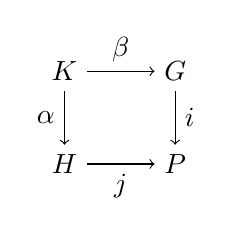
\begin{tikzpicture}[every node/.style={midway}]
			  \matrix[column sep={4em,between origins}, row sep={2em}] at (0,0) {
			    \node(A) {$K$}  ; & \node(Y) {$G$}; \\
			    \node(X) {$H$}; & \node (U) {$P$};\\
			  };
			  \draw[<-] (X) -- (A) node[anchor=east]  {$\alpha$};
			  \draw[->] (A) -- (Y) node[anchor=south] {$\beta$};
			  \draw[->] (Y) -- (U) node[anchor=west] {$i$};
			  \draw[->] (X) --(U) node[anchor=north] {$j$};
		\end{tikzpicture}
	\end{minipage}
	\medskip

	\begin{minipage}{0.5\textwidth}
		Alors par la propriété universelle de l'amalgame il existe un unique morphisme $f : Q \longmapsto P$ tel que $f\circ k = i$ et  $f\circ l = j$ comme sur le diagramme de droite. En échangeant les rôles de $P$ et $Q$ il existe par le même raisonnement un unique morphisme $g : P \longmapsto Q$ faisant commuter le diagramme. On veut montrer que $f$ et $g$ sont inverses l'un de l'autre.	
	\end{minipage}
	\hfill
	\begin{minipage}{0.5\textwidth}
		\[
			\xymatrix@R=1.2cm@C=1.2cm{
			 K \ar[r]^{\beta}      \ar[d]_{\alpha}         & G \ar[d]_{k} \ar@/^1pc/[rdd]^{i}   \\
			 H \ar[r]^{l} \ar@/_1pc/[rrd]_{j} & Q \ar@{-->}[rd]_{\exists! \; f}             \\
							      &                                   & P 
			}
	\]		
	\end{minipage}
	\medskip


	\begin{minipage}{0.5\textwidth}
		On s'intéresse alors à la composition $g\circ f : Q \longmapsto Q$, le raisonnement est encore une fois semblable pour la composition $f\circ g : P \longmapsto P$. Remarquons que $g\circ f$ fait commuter le diagramme suivant, tout comme $Id_Q$, la propriété universelle de l'amalgame garanti l'unicité donc nécessairement $g\circ f = Id_Q$.	
	\end{minipage}
	\hfill
	\begin{minipage}{0.5\textwidth}
		\[
			\xymatrix@R=1.2cm@C=1.2cm{
			 K \ar[r]^{\beta}      \ar[d]_{\alpha}         & G \ar[d]_{k} \ar@/^1pc/[rdd]^{i}   \\
			 H \ar[r]^{l} \ar@/_1pc/[rrd]_{j} & Q \ar@{-->}[rd]_{g\circ f}             \\
							      &                                   & Q 
			}
	\]		
	\end{minipage}
	\medskip

	On obtient finalement bien que $f$ et $g$ son inverses l'un de l'autre ce qui montre que $P$ et $Q$ sont isomorphes. On illustre maintenant cette propriété par quelques exemples.		

	\begin{example}
		\begin{enumerate}
			\item Dans le cas $K = 1$ on a pour $1 \overset{\beta}{\longleftarrow} K \overset{\alpha}{\longrightarrow} G$ 
				 \begin{align*}
					 H*_{1}G &= \quot{H*G}{\alpha(x)\beta(x)^{-1}} \; \forall x \in 1 \\
						 &= \quot{H*G}{\alpha(1)\beta(1)^{-1}} \\
						 &= H*G
				.\end{align*}
				On retrouve le produit libre de $H$ et $G$.
			\item Dans le cas $H = 1$ avec les mêmes morphismes  $\alpha, \beta$ on a 
				\begin{align*}
					1*_K G &= \quot{1*G}{\alpha(x)\beta(x)^{-1}} \; \forall x \in K \\
					       &\cong \quot{G}{\alpha(x)} \\
					       &\cong \quot{G}{N}
				\end{align*}
				où $N$ est le sous groupe normal de $G$ engendré par $K$.
			\item Finalement dans le cas particulier $H=1$ et $K \triangleleft G$ on retrouve $1*G \cong \quot{G}{K}$.
		\end{enumerate}
	\end{example}
\end{document}
